\documentclass[11pt,a4paper]{article}

\usepackage[margin=2.4cm]{geometry}
\usepackage{booktabs}
\usepackage{longtable}
\usepackage{array}
\usepackage{tabularx}
\usepackage{listings}
\usepackage{xcolor}
\usepackage{tikz}
\usepackage{hyperref}
\usepackage{enumitem}
\usepackage{caption}
\usepackage{amsmath}
\usepackage{fancyhdr}
\usetikzlibrary{arrows.meta,positioning,shapes.geometric,fit}

\hypersetup{colorlinks=true,linkcolor=blue!50!black,urlcolor=blue!50!black,citecolor=blue!50!black}
\captionsetup{font=small,labelfont=bf}
\setlist{itemsep=2pt,topsep=3pt}
\lstset{
  basicstyle=\ttfamily\small,
  breaklines=true,
  frame=single,
  rulecolor=\color{gray!40},
  backgroundcolor=\color{gray!5},
  columns=fullflexible,
  keepspaces=true,
  showstringspaces=false
}
\pagestyle{fancy}
\fancyhf{}
\fancyhead[L]{\small NeverFull-NeverStop V11 --- Project Report}
\fancyhead[R]{\small \thepage}
\renewcommand{\headrulewidth}{0.4pt}

\title{\bfseries NeverFull-NeverStop\\[4pt]
\large A Transparent Context-Compaction Proxy for Long-Horizon Agents\\[2pt]
\normalsize V11 Project Report}
\author{Project maintainer \quad \texttt{061115xhsm}}
\date{October 26, 2026 \quad Version V11}

\begin{document}
\maketitle

\begin{abstract}
The bottleneck for long-horizon LLM agents is rarely single-turn reasoning; it is the context window. Once history outgrows the window, an agent either stops or silently loses state. Existing approaches---agent-native compaction (OpenClaw, Claude Code), runtime compressors (Hermes), and engineered memory layers---trade off compression ratio, evidence retention, state consistency, and cost, but they rarely define what a \emph{correct} compression is.

This project implements a transparent proxy between the agent and the model API. V11 shifts the design goal from ``make history shorter'' to ``continue working with verifiable state''. Core mechanisms include reversible context folding (verbatim, addressable archive), commitment/identifier contracts, deterministic evidence probes, a per-session state table, per-model token calibration, a UCB compaction policy, cost attribution, and multi-tenant/multi-instance support. On the same 131-message, $\sim$9k-token coding session with the same summarizer, V11 retained 11/11 gold evidence spans and answered 4/4 reader questions at 0.86 compression, versus 0.64 evidence recall for both OpenClaw and Hermes. Its compaction cost was on par with OpenClaw (9.4k vs 8.9k tokens) and about 82\% of Hermes, with roughly 38\% of Hermes' latency.

The repository ships 88 automated tests (including real PostgreSQL integration, concurrent writes, and streaming pass-through), a CI matrix (Python 3.11--3.13 with a Postgres service), and reproducible evaluation scripts. We also state the limits: single-process caches, SQLite shared-volume constraints, in-process quota counters, and a small evaluation sample.
\end{abstract}

\tableofcontents
\newpage

\section{Introduction}

\subsection{Problem}
A coding or operations agent may run for dozens to hundreds of turns, and tool output---logs, files, web pages---dominates the history. The model context window (128k--1M tokens) caps what can be seen at once. Beyond it, requests fail, get truncated, or are summarized by the agent itself; summaries are unauditable, and constraints, file paths, and failing commands often disappear.

Three mechanisms dominate:
\begin{itemize}
  \item \textbf{Agent-native compaction} (OpenClaw, Claude Code): tightly coupled to memory flushing, tool-pair integrity, and checkpoint replay; compaction happens inside the agent.
  \item \textbf{Runtime compressors} (Hermes): a standalone engine that protects head/tail and summarizes the middle with a cheaper model, triggered by API-reported token usage.
  \item \textbf{Engineered memory layers}: external stores plus retrieval, where a write policy decides what to remember.
\end{itemize}

Their common gap is that \emph{correctness of compression is not verifiable}. Embedding similarity, summary length, and even downstream QA accuracy can hide a broken evidence chain \cite{keepbench,compactbench}.

\subsection{Goals}
The proxy sits between the agent and the upstream API; the agent only points its \texttt{base\_url} at a local port. V11 does not chase the highest compression ratio. It aims for:
\begin{enumerate}
  \item \textbf{Reversibility}: folded history is always retrievable verbatim;
  \item \textbf{Verifiability}: commitments and exact identifiers are checked after compaction and disclosed when missing;
  \item \textbf{State consistency}: current file/decision state is distinguished from superseded state;
  \item \textbf{Operability}: tenant isolation, quotas, encryption, retention, and cost attribution;
  \item \textbf{Measurability}: paired continuation and evidence retention instead of embedding cosine.
\end{enumerate}

\subsection{Contributions}
\begin{itemize}
  \item A reversible folding protocol: typed \texttt{<folded\_context>} placeholders, verbatim archive, pagination, encryption, and key rotation;
  \item Commitment contracts and evidence probes: deterministic scoring (commitments 45\%, identifiers 25\%, sections 15\%, last ask 15\%), with one MUST-PRESERVE retry below the floor;
  \item A session state table: file versions, stale-read marking, and decision supersession---directly targeting ghost memory;
  \item Multi-instance and multi-tenant support: tenant namespaces, a PostgreSQL session store, a Redis shared cache, and per-tenant quotas;
  \item Reproducible three-way and paired evaluations against OpenClaw and Hermes on the same model and transcript.
\end{itemize}

\section{Survey: A Map of 109 Papers}

\subsection{Method}
We queried the arXiv API with 12 topic searches (context compression, agent memory, KV cache, evaluation, RL policies, etc.) and 45 targeted title searches, sorted by submission date. After deduplication, the candidate pool was 550 papers; a whitelist forced canonical works in and a keyword filter removed noise, yielding 109 papers (2023-10 to 2026-10). Data and scripts live under \texttt{research/}.

\begin{table}[htbp]
\centering
\caption{Paper clusters (109 papers)}
\begin{tabular}{lrl}
\toprule
Cluster & Count & Representative work \\
\midrule
Agent memory & 25 & MemGPT, Mem0, MemOS, A-MEM, MIRIX, Memory-R1 \\
Context folding/compaction & 19 & ReFold, REMORY, MemTrace, Compact-Bench, KEEP-Bench \\
Prompt compression & 18 & LLMLingua/2, LongLLMLingua, RECOMP, ICAE, COMI \\
Evaluation & 13 & LongMemEval, LoCoMo, RULER, HELMET, NoLiMa \\
Retrieval & 7 & HippoRAG, Infinite Retrieval, Organize-then-Retrieve \\
Structured state & 5 & TEM, Narrative State Tracking \\
Long/streaming & 5 & Titans, MoBA, Quest \\
KV cache & 4 & SnapKV, MInference, Native Sparse Attention \\
RL policies & 2 & Memory-R2, Uni-Mem \\
Surveys & 4 & Context Engineering Survey, Agent Memory Survey \\
Other & 6 & --- \\
\bottomrule
\end{tabular}
\end{table}

\subsection{Findings}
\begin{enumerate}
  \item \textbf{Summaries are being replaced by folding.} ReFold \cite{refold} shows training-free, reversible inter-turn folding beats predictive triggering; MemTrace \cite{memtrace} shows repository changes invalidate earlier evidence, so compaction must be state-consistent.
  \item \textbf{Correctness equals commitment preservation.} ``Compress the Context, Keep the Commitments'' \cite{commitments} defines context as a set of commitments; KEEP-Bench \cite{keepbench} shows QA metrics underestimate unfaithful compression.
  \item \textbf{Evaluation must be paired.} Compact-Bench \cite{compactbench} compares full-history and summary-only continuations from the same repository state, avoiding false positives from lucky summaries.
  \item \textbf{Flattening structure is a security hole.} Compaction Laundering \cite{laundering} shows that collapsing typed conversations into plain text destroys provenance; folded placeholders must keep types and references.
  \item \textbf{Evolving state is harder than fact recall.} \cite{evolving,atma} name ghost memory: old, current, and transitional facts coexist and contaminate retrieval.
  \item \textbf{With strong models, design less and retrieve more.} MemoryTax \cite{memorytax} and Skip the Compressor \cite{skipcompressor} show that when a model can search raw history itself, pre-built memory pipelines yield little; light folding plus searchable history often wins.
\end{enumerate}

\section{Architecture}

\subsection{Position in the Request Path}
The proxy is transparent to the agent. It maintains side stores for archives, state, and sessions, and exposes health and metrics.

\begin{figure}[htbp]
\centering
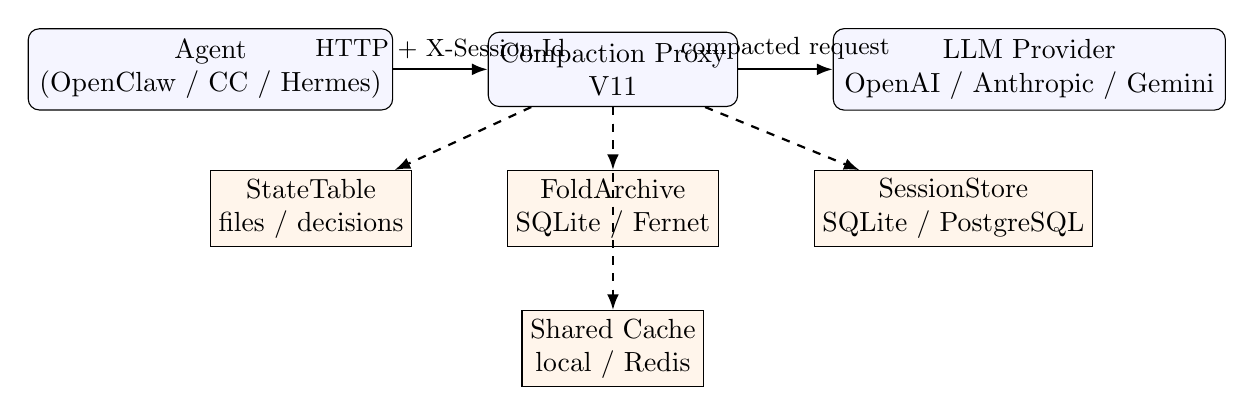
\begin{tikzpicture}[
  node distance=8mm and 12mm,
  box/.style={draw,rounded corners,align=center,minimum height=8mm,inner sep=4pt,fill=blue!4},
  store/.style={draw,align=center,minimum height=7mm,inner sep=3pt,fill=orange!8},
  arr/.style={-{Latex[length=2mm]},thick}
]
\node[box] (agent) {Agent\\(OpenClaw / CC / Hermes)};
\node[box,right=of agent] (proxy) {Compaction Proxy\\V11};
\node[box,right=of proxy] (up) {LLM Provider\\OpenAI / Anthropic / Gemini};
\node[store,below=of proxy] (fold) {FoldArchive\\SQLite / Fernet};
\node[store,left=of fold] (state) {StateTable\\files / decisions};
\node[store,right=of fold] (sess) {SessionStore\\SQLite / PostgreSQL};
\node[store,below=of fold] (cache) {Shared Cache\\local / Redis};
\draw[arr] (agent) -- node[above,font=\small]{HTTP + X-Session-Id} (proxy);
\draw[arr] (proxy) -- node[above,font=\small]{compacted request} (up);
\draw[arr,dashed] (proxy) -- (fold);
\draw[arr,dashed] (proxy) -- (state);
\draw[arr,dashed] (proxy) -- (sess);
\draw[arr,dashed] (proxy) -- (cache);
\end{tikzpicture}
\caption{Proxy position and side stores}
\end{figure}

\subsection{Request Lifecycle}
\begin{enumerate}
  \item \textbf{Tenant and identity}: middleware reads \texttt{X-Tenant-Id}; \texttt{extract\_session\_id} produces a tenant-scoped id (e.g., \texttt{acme:s1}) and echoes it in response headers.
  \item \textbf{Budget and trigger}: CJK-aware estimation (fast + accurate) corrected by a per-model factor; exceeding the effective threshold (default 80\%, weak/strong/auto profiles) triggers proactive compaction; upstream overflow errors trigger recovery.
  \item \textbf{Policy}: a UCB bandit keyed by task class and tenant chooses light/standard/deep, mapping to retained turns.
  \item \textbf{Pipeline}: tool-output pruning $\rightarrow$ commitment/identifier extraction $\rightarrow$ submodular selection $\rightarrow$ parallel or single-block summary $\rightarrow$ fold archive $\rightarrow$ contract verification $\rightarrow$ evidence probes (retry once below 0.75).
  \item \textbf{Assembly}: state snapshot + folded placeholder + sectioned summary + last six turns; tool-pair integrity is enforced before forwarding.
  \item \textbf{Metering}: upstream \texttt{usage} is recorded for cost, savings, and latency; daily tenant budgets are updated.
\end{enumerate}

\subsection{Modules}
\begin{table}[htbp]
\centering
\caption{Core modules (tests and benchmark scripts excluded)}
\begin{tabular}{lrl}
\toprule
Module & LOC & Responsibility \\
\midrule
\texttt{compaction-proxy.py} & 8,273 & HTTP service, pipeline, stores, routing \\
\texttt{folding.py} & 517 & archive, digest, placeholder, contract, encryption/rotation \\
\texttt{state\_table.py} & 304 & file/decision state, stale marking, prune \\
\texttt{evidence.py} & 111 & four-dimensional evidence probes \\
\texttt{policy.py} & 170 & task classifier, UCB policy, capability profiles \\
\texttt{calibration.py} & 68 & per-model token calibration \\
\texttt{cost\_tracker.py} & 96 & per-request ring buffer, daily quota \\
\texttt{tenant.py} & 29 & tenant context and namespacing \\
\texttt{shared\_cache.py} & 71 & Redis/local compaction cache \\
\texttt{session\_store\_pg.py} & 250 & PostgreSQL session store \\
\bottomrule
\end{tabular}
\end{table}

\section{Mechanisms}

\subsection{Reversible Folding}
Compaction no longer returns a free-text summary alone:
\begin{enumerate}
  \item old messages are written \emph{verbatim} to an archive (SQLite WAL), addressed as \texttt{fold:<hash>} where the hash includes tenant and content;
  \item a deterministic digest is computed: message count, roles, tools, files, commands, errors, commitments;
  \item a typed placeholder preserves provenance and a retrievable reference.
\end{enumerate}

\begin{lstlisting}
<folded_context ref="fold:6f775980e76a" messages="31" approx_tokens="8120">
[FOLD] 31 messages elided (user 14 / assistant 17)
[TOOLS] execx9, editx4, readx7
[FILES] /tmp/proj/src/core.py, /tmp/proj/config.yaml
[COMMANDS] pytest -q; npm test
[OBSERVED] 3 error/failure mentions
[COMMITMENTS] decision=2, constraint=1, task=1
[RETRIEVE] GET /fold/fold:6f775980e76a returns the original messages verbatim.
</folded_context>
\end{lstlisting}

The archive supports paginated retrieval (\texttt{offset/limit}, default 200, cap 500), optional Fernet encryption (key 0600), key rotation (\texttt{POST /maintenance/rotate-key}), and retention by tenant, age, and count.

\subsection{Commitment Contracts and Evidence Probes}
Before compaction, commitments (goals, constraints, decisions, errors, file operations, tasks) and exact identifiers (paths, function names, error fragments) are extracted. After compaction:
\begin{equation}
S = 0.45\,S_{\text{commit}} + 0.25\,S_{\text{id}} + 0.15\,S_{\text{sections}} + 0.15\,S_{\text{ask}} .
\end{equation}
Below the floor $\tau=0.75$, one retry is made with an explicit MUST-PRESERVE list; the better result is kept. Anything still missing is disclosed in \texttt{<unpreserved\_commitments>} rather than silently lost.

\subsection{State Table}
Each session keeps a file table (path, last operation, timestamp, edit/read counts) and a decision table (goal/constraint/decision/task, active/superseded), rendered as:
\begin{lstlisting}
<state_snapshot>
[FILES] /tmp/proj/config.yaml (edit 10:32; earlier reads stale)
[DECISIONS] active: (decision) use sqlite for cache ; superseded: 1
[NOTE] Treat earlier reads of edited files as stale; re-read before relying.
</state_snapshot>
\end{lstlisting}
This targets MemTrace-style consistency and A-TMA-style ghost memory.

\subsection{Policy and Calibration}
A UCB1 bandit selects an action per task class:
\begin{equation}
a_t = \arg\max_a \left( \bar r_a + \sqrt{\frac{2\ln N}{n_a}} \right),
\end{equation}
with a forced \texttt{light} action when the session's evidence EMA falls below the performance floor. Token calibration learns $f \leftarrow 0.8f + 0.2\,(\text{actual}/\text{estimated})$, clamped to $[0.5,2.0]$, correcting CJK heuristics against the provider tokenizer.

\subsection{Cost Attribution}
Provider \texttt{usage} is preferred (OpenAI \texttt{prompt\_tokens}, Anthropic \texttt{input\_tokens}, Gemini \texttt{promptTokenCount}); the proxy records cost, savings, latency, cache hits, and tenant per compaction, falling back to estimation when usage is absent. \texttt{/health.cost\_recent} aggregates by model and tenant with p50/p95 latency.

\section{Multi-Instance and Multi-Tenant}

\subsection{Tenant Isolation}
\texttt{X-Tenant-Id} is normalized into the request context; session ids become \texttt{tenant:session}, partitioning sessions, state, cost, and rate-limit buckets. Fold archives store \texttt{tenant\_id}; cross-tenant retrieval returns 404; ref hashes include the tenant so identical content cannot overwrite another tenant's archive.

\subsection{Shared Storage}
\begin{itemize}
  \item \textbf{PostgreSQL SessionStore}: sessions, prior summaries, transcripts, and ARC entries live in Postgres for cross-instance reads; search uses Postgres full-text with an ILIKE fallback; rows are trimmed per tenant.
  \item \textbf{Redis compaction cache}: with \texttt{COMPACTION\_PROXY\_REDIS\_URL}, summaries use \texttt{SETEX} keyed by tenant and history hash; otherwise the process-local cache is used.
  \item \textbf{Instance identity}: \texttt{COMPACTION\_PROXY\_INSTANCE\_ID} and \texttt{X-Instance-Id}; \texttt{MAINTENANCE\_OWNER} restricts periodic cleanup to one instance.
\end{itemize}

\subsection{Quotas}
Per-tenant caps on archives, sessions, and daily tokens are enforced on write (oldest trimmed) and, with \texttt{ENFORCE\_QUOTA=1}, by skipping compaction once the daily budget is exhausted---preventing one tenant from draining a shared upstream.

\section{Security and Operations}

\begin{table}[htbp]
\centering
\caption{Security and operations}
\begin{tabularx}{\linewidth}{lX}
\toprule
Capability & Implementation \\
\midrule
Authentication & \texttt{REQUIRE\_AUTH=1} refuses to start without an API secret (fail-closed); endpoints use \texttt{require\_auth} \\
Rate limiting & Token bucket per \texttt{tenant:ip}; disabled by default, configurable per minute \\
Body size & Request cap (default 2 MB), 413 beyond \\
Encryption & Optional Fernet for folded payloads; key file 0600; rotation endpoint re-encrypts all rows \\
Retention & Age and row caps for folds/state/sessions; runs every 100 compactions; \texttt{/maintenance/prune} manual trigger \\
Observability & \texttt{/health} (storage, quotas, encryption, cost, p50/p95), \texttt{/metrics} (Prometheus) \\
\bottomrule
\end{tabularx}
\end{table}

\section{Evaluation}

\subsection{Three-Way Comparison}
On the same 131-message, $\sim$9,087-token coding session, with the same summarizer (local \texttt{tierflow\_pro}) and the same four-question reader, we compared OpenClaw (prompt and cut policy reproduced from v2026.10.5), Hermes (the real \texttt{ContextCompressor}, aux LLM replaced by the same endpoint), and V11.

\begin{table}[htbp]
\centering
\caption{Three-way compaction comparison (single run)}
\begin{tabular}{lccccc}
\toprule
System & Compression & Evidence recall & State & QA & Cost (tokens) \\
\midrule
OpenClaw & 0.491 & 0.636 & 0.5 & 3/4 & 8,934 \\
Hermes & 0.471 & 0.636 & 1.0 & 3/4 & 11,410 \\
\textbf{NeverFull V11} & \textbf{0.860} & \textbf{1.000} & \textbf{1.0} & \textbf{4/4} & 9,369 \\
\bottomrule
\end{tabular}
\end{table}

Latency: OpenClaw 18.3 s, Hermes 67.7 s, V11 25.5 s. All three preserved decisions and paths, but only V11 preserved the failing-test command \texttt{pytest -q}---an evidence-chain difference, not merely an answer-accuracy one. OpenClaw did not mark the earlier config read as stale; Hermes was the most expensive and slowest.

\subsection{Paired Evaluation}
\texttt{benchmark/paired\_eval.py} builds full, truncate, summary, and fold views of the same conversation and measures compression and evidence recall against identical probes. On synthetic data the fold view reaches 92.2\% compression at 1.000 evidence recall; truncation reaches 65.0\% at 1.000 (because answers sit at the tail), illustrating that the metric distinguishes \emph{what survived}, not just length.

\subsection{Supplementary: LoCoMo Memory Benchmark (4 conversations)}
Beyond the coding session, we evaluated four long LoCoMo conversations (four category-stratified questions each, 16 total). With the same summarizer, a generic summary reaches 98.0\% compression but retains only 0.199 evidence; V11 reaches 92.1\% compression and retains 0.919 (on par with 65\% truncation), with QA 0.167 (full-context ceiling 0.500; the local reader's temporal reasoning is the bottleneck). conv-41 summaries timed out twice and were skipped (resilience), so llm/v11 rows have views=3. Details: \texttt{research/EVAL-2026-10-26.md}.

\begin{table}[htbp]
\centering
\caption{Supplementary LoCoMo evaluation (4 conversations x 4 questions)}
\begin{tabular}{lcccc}
\toprule
Strategy & Compression & Evidence & QA & Summary time/conv \\
\midrule
full & 0.000 & 0.979 & 0.500 & 0 s \\
truncate & 0.650 & 0.948 & 0.125 & 0 s \\
generic LLM summary & 0.980 & 0.199 & 0.083 & 11.3 s \\
\textbf{V11 fold} & \textbf{0.921} & \textbf{0.919} & \textbf{0.167} & 16.0 s \\
\bottomrule
\end{tabular}
\end{table}

\subsection{Tests and Stress}
\begin{table}[htbp]
\centering
\caption{Verification results}
\begin{tabularx}{\linewidth}{lX}
\toprule
Item & Result \\
\midrule
Unit/integration tests & 88 passing (6 real-PostgreSQL, concurrency, streaming pass-through, key rotation, quotas) \\
Concurrent writes & Before the fix: 78/320 and 116/320 errors under 8 threads; after locks and \texttt{busy\_timeout}: 0 \\
HTTP health & 100 sequential p50 1 ms; 200 concurrent in 0.09 s, all successful \\
Error paths & Malformed JSON 400; 1.5 MB body 413; upstream down 502; process stays alive \\
\bottomrule
\end{tabularx}
\end{table}

\subsection{Limitations}
\begin{itemize}
  \item One synthetic conversation, four questions, one run; conclusions are directional and need LongMemEval/LoCoMo and multi-task paired sets.
  \item OpenClaw is a source-level reproduction, not a live Gateway session; its \texttt{keepRecentTokens} was scaled for the test.
  \item Cost uses measured \texttt{usage}; cache benefits and network overhead are not included.
\end{itemize}

\section{Engineering}

The V11 iteration produced eight main commits:
\begin{lstlisting}
75893e9  P0+P1a: baseline, tests/CI, session-id, reversible folding
4ef1cb6  P1b-P5: state table, evidence, paired eval, policy, cost
b52d5b4  three-way benchmark (OpenClaw / Hermes / NeverFull)
9a53c9b  sqlite thread-safety fix + concurrency tests
8779806  ops pass: retention, auth/rate limits, encryption, calibration
d7a4574  cost tracker, key rotation, streaming test, docs
5f7cc44  tenant isolation, shared cache, instance identity
fba1a7a  PostgreSQL SessionStore, quotas, rotate-key endpoint
\end{lstlisting}

CI runs Python 3.11--3.13 with a Postgres service, byte-compiles entrypoints, runs 88 tests, and executes the paired evaluation. Dependencies are minimal: only \texttt{aiohttp} at runtime; Postgres, Redis, and semantic models are optional.

\section{Future Work}
\begin{enumerate}
  \item \textbf{Scale evaluation}: add LongMemEval, LoCoMo, and Compact-Bench to CI with a real LLM reader and multi-task paired sets.
  \item \textbf{Cache-aware compaction}: avoid rewriting the prefix every time and account for prompt-cache hits.
  \item \textbf{Multi-instance consistency}: share policy/calibration in Redis and stress-test sticky routing and failover.
  \item \textbf{Durable quotas}: persist daily budgets across restarts and export per-tenant billing.
  \item \textbf{Learned policies}: replace the UCB bandit with a policy trained on task success and cost.
\end{enumerate}

\section{Conclusion}
V11 moves context compression from ``shorter summaries'' to ``verifiably continuing work'': folding keeps the original reversible, contracts and probes verify commitments, the state table prevents stale evidence, and tenants/quotas make it operable. In a three-way test with the same model and comparable cost, it clearly led on evidence retention and task continuation. The project is still single-process-centric, but its mechanisms and evaluation harness are ready to scale.

\appendix
\section{Key Configuration}
\begin{longtable}{p{6.2cm}p{8.2cm}}
\toprule
Variable & Purpose \\
\midrule
\texttt{COMPACTION\_PROXY\_FOLDING} & Enable reversible folding (default 0) \\
\texttt{COMPACTION\_PROXY\_CONTRACT\_RETRY} & Retry on weak evidence (default 1) \\
\texttt{COMPACTION\_PROXY\_EVIDENCE\_FLOOR} & Evidence floor (default 0.75) \\
\texttt{COMPACTION\_PROXY\_POLICY} & Enable UCB policy (default 0) \\
\texttt{COMPACTION\_PROXY\_AGENT\_PROFILE} & weak/strong/auto threshold profile \\
\texttt{COMPACTION\_PROXY\_STRICT\_SESSION} & Refuse content-fingerprint session ids \\
\texttt{COMPACTION\_PROXY\_STORAGE} & sqlite/postgres \\
\texttt{COMPACTION\_PROXY\_PG\_DSN} & PostgreSQL DSN \\
\texttt{COMPACTION\_PROXY\_REDIS\_URL} & Shared compaction cache \\
\texttt{COMPACTION\_PROXY\_TENANT\_MAX\_FOLDS} & Per-tenant archive cap \\
\texttt{COMPACTION\_PROXY\_TENANT\_MAX\_SESSIONS} & Per-tenant session cap \\
\texttt{COMPACTION\_PROXY\_TENANT\_DAILY\_TOKENS} & Per-tenant daily token budget \\
\texttt{COMPACTION\_PROXY\_ENFORCE\_QUOTA} & Skip compaction when over budget \\
\texttt{COMPACTION\_PROXY\_FOLD\_ENCRYPT} & Archive encryption \\
\texttt{COMPACTION\_PROXY\_RETENTION\_DAYS} & Retention window \\
\texttt{COMPACTION\_PROXY\_RATE\_LIMIT} & Requests per minute per IP \\
\texttt{COMPACTION\_PROXY\_REQUIRE\_AUTH} & Fail closed without a secret \\
\bottomrule
\end{longtable}

\section{Reproduction}
\begin{lstlisting}[language=bash]
# tests
python -m unittest discover -s tests -v

# paired evaluation
python benchmark/paired_eval.py --limit 3

# three-way comparison (requires a local OpenAI-compatible endpoint)
python benchmark/compare_systems.py --json research/data/compare.json

# run with folding + policy + encryption
COMPACTION_PROXY_FOLDING=1 COMPACTION_PROXY_FOLD_ENCRYPT=1 \
COMPACTION_PROXY_POLICY=1 COMPACTION_PROXY_AGENT_PROFILE=auto \
python compaction-proxy.py
\end{lstlisting}

\section{Selected References}
\begin{thebibliography}{99}
\bibitem{refold} ReFold: Training-Free Reversible Inter-Turn Context Folding for Long-Horizon Agents. arXiv:2610.07863.
\bibitem{commitments} Compress the Context, Keep the Commitments: A Formal Framework for Verifiable LLM Context Compression. arXiv:2605.17304.
\bibitem{keepbench} KEEP-Bench: Evaluating Evidence Preservation in Context Compression. arXiv:2610.26827.
\bibitem{compactbench} Compact-Bench: Measuring What Context Compaction Costs Long-Horizon Coding Agents. arXiv:2610.31710.
\bibitem{laundering} Compaction Laundering: Provenance Destruction in Context-Compacting Coding Agents. arXiv:2610.29869.
\bibitem{memtrace} MemTrace: State-Consistent Memory for Long-Horizon Coding Agents. arXiv:2610.04838.
\bibitem{atma} A-TMA: Decoupling State-Aware Memory Failures in Long-Term Agent Memory. arXiv:2607.01935.
\bibitem{evolving} Can Agent Memory Systems Track Evolving State? arXiv:2608.19652.
\bibitem{memorytax} MemoryTax: The Bitter Lesson of Agent Memory. arXiv:2610.29823.
\bibitem{skipcompressor} Skip the Compressor: Coding Agents Fix More Issues When They Pick Whole Files. arXiv:2610.21073.
\bibitem{prunesummary} Prune the Summary, Not the History: Source-Judged Compaction for Long-Horizon Agents. arXiv:2610.20927.
\bibitem{transparency} Maximising Transparency in Context Compaction Improves Retention of Facts and Commitments. arXiv:2610.20116.
\bibitem{progressgraphs} Persistent Context Graphs for Efficient Memory Compaction in LLM Agents. arXiv:2609.40118.
\bibitem{memoryr1} Memory-R1: Enhancing Large Language Model Agents to Manage and Utilize Memories via Reinforcement Learning. arXiv:2508.19828.
\bibitem{memagent} MemAgent: Reshaping Long-Context LLM with Multi-Conv RL-based Memory Agent. arXiv:2507.02259.
\bibitem{mem0} Mem0: Building Production-Ready AI Agents with Scalable Long-Term Memory. arXiv:2504.19413.
\bibitem{longmemeval} LongMemEval: Benchmarking Chat Assistants on Long-Term Interactive Memory. arXiv:2410.10813.
\bibitem{locomo} Evaluating Very Long-Term Conversational Memory of LLM Agents. arXiv:2402.17753.
\bibitem{ruler} RULER: What's the Real Context Size of Your Long-Context Language Models? arXiv:2404.06654.
\bibitem{llmlingua} LLMLingua: Compressing Prompts for Accelerated Inference of Large Language Models. arXiv:2310.05736.
\end{thebibliography}

\end{document}
